\section*{Appendix}

\begin{subappendices}
\section{Parameter Estimation}
\label{c4:appendix:param_estimation}
We estimate the parameters of the joint model using Markov chain Monte Carlo (MCMC) methods under the Bayesian framework. Let~$\boldsymbol{\theta}$ denote the vector of all of the parameters of the joint model. The joint model postulates that given the random effects, the time to progression, and all of the longitudinal measurements taken over time are all mutually independent. Under this assumption the posterior distribution of the parameters is given by:
\begin{align*}
p(\boldsymbol{\theta}, \boldsymbol{b} \mid \mathcal{D}_n) & \propto \prod_{i=1}^n p(l_i, r_i, \boldsymbol{y}_{1i},\ldots \boldsymbol{y}_{Ki}, \mid \boldsymbol{b}_i, \boldsymbol{\theta}) p(\boldsymbol{b}_i \mid \boldsymbol{\theta}) p(\boldsymbol{\theta})\\
& \propto \prod_{i=1}^n \prod_{k=1}^K p(l_i, r_i \mid \boldsymbol{b}_i, \boldsymbol{\theta})  p(\boldsymbol{y}_{ki} \mid \boldsymbol{b}_{i}, \boldsymbol{\theta}) p(\boldsymbol{b}_i \mid \boldsymbol{\theta}) p(\boldsymbol{\theta}),\\
p(\boldsymbol{b}_i \mid \boldsymbol{\theta}) &= \frac{1}{\sqrt{(2 \pi)^{\mid W \mid} \text{det}(\boldsymbol{D})}} \exp(\boldsymbol{b}_i^{\top} \boldsymbol{D}^{-1} \boldsymbol{b}_i),
\end{align*}
where, the likelihood contribution of the~${k\mbox{-th}}$ longitudinal outcome vector~$\boldsymbol{y}_{ki}$ for the~${i\mbox{-th}}$ patient, conditional on the random effects is:
\begin{equation*}
p(\boldsymbol{y}_{ki} \mid \boldsymbol{b}_i, \boldsymbol{\theta}) = \prod_{j=1}^{n_{ki}} \exp\Bigg[\frac{y_{kij} \psi_{kij}(\boldsymbol{b}_{ki}) - c_k\big\{\psi_{kij}(\boldsymbol{b}_{ki})\big\}}{a_k(\varphi)} - d_k(y_{kij}, \varphi)\Bigg],
\end{equation*}
where~$n_{ki}$ are the total number of longitudinal measurements of type~$k$ for patient~$i$. The natural and dispersion parameters of the exponential family are denoted by~$\psi_{kij}(\boldsymbol{b}_{ki}$ and~$\varphi$, respectively. In addition,~$c_k(\cdot), a_k(\cdot), d_k(\cdot)$ are known functions specifying the member of the exponential family. The likelihood contribution of the time to progression outcome is given by:
\begin{equation}
\begin{split}
\label{c4:eq:likelihood_contribution_survival}
p(l_i,r_i\mid \boldsymbol{b}_i,\boldsymbol{\theta}) &= \exp\Big[-\int_0^{l_i} h_i\big\{s \mid \mathcal{M}_i(t), \boldsymbol{w}_i(t)\big\}\mathrm{d}{s}\Big]\\ & \quad - \exp\Big[-\int_0^{r_i}h_i\big\{s \mid \mathcal{M}_i(t), \boldsymbol{w}_i(t)\big\}\mathrm{d}{s}\Big].
\end{split}
\end{equation}
The integral in~(\ref{c4:eq:likelihood_contribution_survival}) does not have a closed-form solution, and therefore we use a 15-point Gauss-Kronrod quadrature rule to approximate it.

We use independent normal priors with zero mean and variance 100 for the fixed effect parameters of the longitudinal model. For scale parameters we inverse Gamma priors. For the variance-covariance matrix~$\boldsymbol{D}$ of the random effects we take inverse Wishart prior with an identity scale matrix and degrees of freedom equal to the total number of random effects. For the relative risk model's parameters~$\boldsymbol{\gamma}$ and the association parameters~$\boldsymbol{\alpha}$, we use independent normal priors with zero mean and variance 100. However, when~$\boldsymbol{\alpha}$ becomes high dimensional (e.g., when several functional forms are considered per longitudinal outcome), we opt for a global-local ridge-type shrinkage prior, i.e., for the s-th element of~$\boldsymbol{\alpha}$ we assume:
\begin{equation}
\alpha_s \sim \mathcal{N}(0, \tau \psi_s),\, \tau^{-1} \sim \mbox{Gamma} (0.1,0.1), \, \psi_s^{-1} \sim \mbox{Gamma}(1, 0.01).
\end{equation}
The global smoothing parameter~$\tau$ has sufficiently mass near zero to ensure shrinkage, while the local smoothing parameter~$\psi_s$ allows individual coefficients to attain large values. Other options of shrinkage or variable-selection priors could be used as well~\citep{andrinopoulou2016bayesian}. Finally, the penalized version of the B-spline approximation to the
baseline hazard is specified using the following hierarchical prior for~$\gamma_{h_0}$~\citep{lang2004bayesian}:
\begin{equation}
p(\gamma_{h_0} \mid \tau_h) \propto \tau_h^{\rho(\boldsymbol{K})/2} \exp\Big(-\frac{\tau_h}{2}\gamma_{h_0}^{\top}\boldsymbol{K}\gamma_{h_0}\Big)
\end{equation}
where~$\tau_h$ is the smoothing parameter that takes a~$\mbox{Gamma}(1, \tau_{h\delta})$ prior distribution, with a hyper-prior~$\tau_{h\delta} \sim \mbox{Gamma}(10^{-3}, 10^{-3})$, which ensures a proper posterior distribution for~$\gamma_{h_0}$~\citep{jullion2007robust},~$\boldsymbol{K} = \Delta_r^{\top} \Delta_r + 10^{-6} \boldsymbol{I}$, with~$\Delta_r$ denoting the~${r\mbox{-th}}$ difference penalty matrix, and~$\rho(\boldsymbol{K})$ denotes the rank of~$\boldsymbol{K}$.

\section{Joint Model for the PRIAS Dataset Used in Simulation Study}
In this work, we reused a joint model we previously fitted to the PRIAS dataset~\citep{tomer2019personalized,tomer2020webapp}. The PRIAS database is not openly accessible. However, access to the database can be requested on the basis of a study proposal approved by the PRIAS steering committee. The website of the PRIAS program is \url{www.prias-project.org}. For the sake of completeness and reproducibility of results, we have presented the PRIAS based model's definition and parameter estimates below. Figure~\ref{c4:fig:app1} shows the cumulative-risk of progression over the follow-up period.

\begin{figure}
\centerline{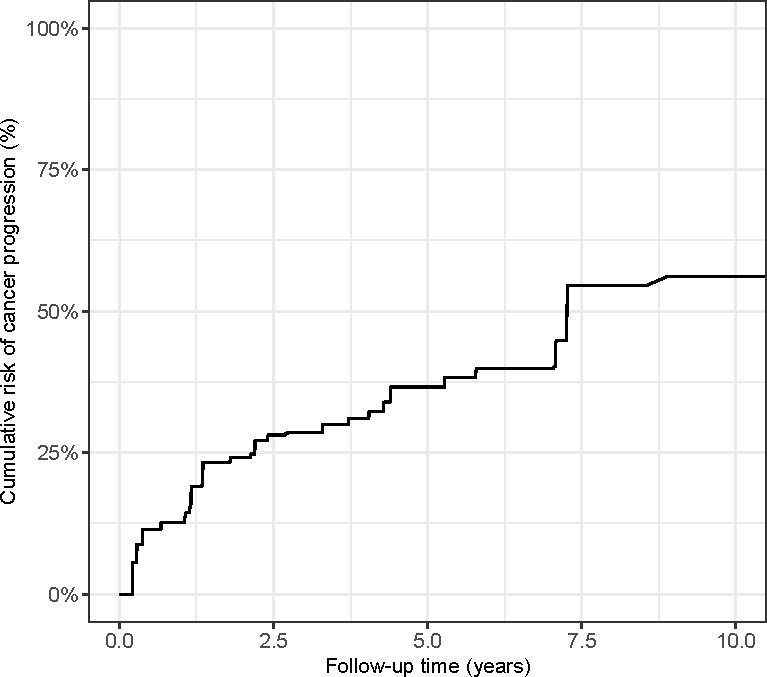
\includegraphics{contents/c4/images/c4_fig_app1.pdf}}
\caption{\textbf{Estimated cumulative-risk of cancer progression~\citep{tomer2020webapp}} for patients in the Prostate Cancer Research International Active Surveillance (PRIAS) dataset. Nearly 50\% patients (\emph{slow progressing}) do not progress in the ten year follow-up period. Cumulative-risk is estimated using nonparametric maximum likelihood estimation~\citep{turnbull1976empirical}, to account for interval censored progression times observed in the PRIAS dataset. Censoring includes death, removal from surveillance on the basis of observed longitudinal data, and patient dropout.}
\label{c4:fig:app1}
\end{figure}

\subsection{Model Specification}
\label{c4:appendix:prias_model}
Let~$T_i^*$ denote the true progression time of the~${i\mbox{-th}}$ patient included in PRIAS. Since biopsies are conducted periodically,~$T_i^*$ is observed with interval censoring~${l_i < T_i^* \leq r_i}$. When progression is observed for the patient at his latest biopsy time~$r_i$, then~$l_i$ denotes the time of the second latest biopsy. Otherwise,~$l_i$ denotes the time of the latest biopsy and~${r_i=\infty}$. Let~$\boldsymbol{y}_{di}$ and~$\boldsymbol{y}_{pi}$ denote his observed DRE (digital rectal examination) and PSA (prostate-specific antigen) longitudinal measurements, respectively. The observed data of all~$n$ patients is denoted by~${\mathcal{D}_n = \{l_i, r_i, \boldsymbol{y}_{di}, \boldsymbol{y}_{pi}; i = 1, \ldots, n\}}$.

The patient-specific DRE and PSA measurements over time are modeled using a bivariate generalized linear mixed effects sub-model. The sub-model for DRE is given by:
\begin{equation}
\label{c4:eq:long_model_dre}
\begin{split}
    \mbox{logit} \big[\mbox{Pr}\{y_{di}(t) > \mbox{T1c}\}\big] &= \beta_{0d} + b_{0di} + (\beta_{1d} + b_{1di}) t\\
    &+ \beta_{2d} (\mbox{Age}_i-65) + \beta_{3d} (\mbox{Age}_i-65)^2
    \end{split}
\end{equation}
where,~$t$ denotes the follow-up visit time, and~$\mbox{Age}_i$ is the age of the~${i\mbox{-th}}$ patient at the time of inclusion in AS. The fixed effect parameters are denoted by~${\{\beta_{0d}, \ldots, \beta_{3d}\}}$, and~${\{b_{0di}, b_{1di}\}}$ are the patient specific random effects. With this definition, we assume that the patient-specific log odds of obtaining a DRE measurement larger than T1c (palpable tumor) remain linear over time. 

The mixed effects sub-model for PSA is given by:
\begin{equation}
\label{c4:eq:long_model_psa}
\begin{split}
    \log_2 \big\{y_{pi}(t) + 1\big\} &= m_{pi}(t) + \varepsilon_{pi}(t),\\
    m_{pi}(t) &= \beta_{0p} + b_{0pi} + \sum_{k=1}^3 (\beta_{kp} + b_{kpi})  B_k(t,\mathcal{K})\\ 
    &+ \beta_{4p} (\mbox{Age}_i-65) + \beta_{5p} (\mbox{Age}_i-65)^2,
    \end{split}
\end{equation}
where,~$m_{pi}(t)$ denotes the underlying measurement error free value of the $\log_2 (\mbox{PSA} + 1)$ transformed \citep{tomer2019personalized} measurements at time~$t$. We model it non-linearly over time using B-splines~\citep{de1978practical}. To this end, the B-spline basis function~$B_k(t, \mathcal{K})$ has two internal knots at~$\mathcal{K} = \{0.75, 2.12\}$ years (33-rd and 66-th percentile of observed follow-up times), and boundary knots at 0 and 6.4 years (95-th percentile of the observed follow-up times). The fixed effect parameters are denoted by~${\{\beta_{0p},\ldots,\beta_{5p}\}}$, and~${\{b_{0pi}, \ldots, b_{3pi}\}}$ are the patient specific random effects. The error~$\varepsilon_{pi}(t)$ is assumed to be t-distributed with three degrees of freedom~\citep{tomer2019personalized} and scale~$\sigma$, and is independent of the random effects. 

To account for the correlation between the DRE and PSA measurements of a patient, link their corresponding random effects are linked. Specifically, the complete vector of random effects~${\boldsymbol{b}_i = (b_{0di}, b_{1di}, b_{0pi}, \ldots, b_{3pi})^\top}$ is assumed to follow a multivariate normal distribution with mean zero and variance-covariance matrix~$\boldsymbol{W}$.

To model the impact of DRE and PSA measurements on the risk of progression, the joint model uses a relative risk sub-model. More specifically, the hazard of progression~$h_i(t)$ at a time~$t$ is given by:
\begin{equation}
\label{c4:eq:rel_risk_model}
\begin{split}
    h_i(t) &= h_0(t) \exp\Big(\gamma_1 (\mbox{Age}_i-65) + \gamma_2 (\mbox{Age}_i-65)^2\\
    &+\alpha_{1d} \mbox{logit} \big[\mbox{Pr}\{y_{di}(t) > \mbox{T1c}\}\big]+ \alpha_{1p} m_{pi}(t) + \alpha_{2p} \frac{\partial m_{pi}(t)}{\partial {t}}\Big),
    \end{split}
\end{equation}
where,~$\gamma_1, \gamma_2$ are the parameters for the effect of age. The parameter~$\alpha_{1d}$ models the impact of log odds of obtaining a~$\mbox{DRE} > \mbox{T1c}$ on the hazard of progression. The impact of PSA on the hazard of progression is modeled in two ways: a) the impact of the error free underlying PSA value~$m_{pi}(t)$, and b) the impact of the underlying PSA velocity~$\partial m_{pi}(t)/\partial {t}$. The corresponding parameters are~$\alpha_{1p}$ and~$\alpha_{2p}$, respectively. Lastly,~$h_0(t)$ is the baseline hazard at time t, and is modeled flexibly using P-splines~\citep{eilers1996flexible}.

\subsection{Parameter Estimates}
\label{c4:appendix:param_estimates}
The posterior parameter estimates for the PRIAS based joint model are shown in Table~\ref{c4:tab:DRE_long} (longitudinal sub-model for DRE outcome), Table~\ref{c4:tab:PSA_long} (longitudinal sub-model for PSA outcome) and Table~\ref{c4:tab:DRE_PSA_survival} (relative risk sub-model). The parameter estimates for the variance-covariance matrix~$\boldsymbol{W}$ from the longitudinal sub-model are shown in the following Table~\ref{c4:tab:D_matrix}:

\begin{table}
\small
\centering
\caption{Estimated variance-covariance matrix~$\boldsymbol{W}$ of the random effects~${\boldsymbol{b}=(b_{0d},b_{1d},b_{0p}, b_{1p}, b_{2p}, b_{3p})}$ from the joint model fitted to the PRIAS dataset.}
\label{c4:tab:D_matrix}
\begin{tabular}{lrrrrrr}
\toprule
Random Effects    & $b_{0d}$    & $b_{1d}$    & $b_{0p}$    & $b_{1p}$   & $b_{2p}$   & $b_{3p}$ \\
\midrule
$b_{0d}$ & 9.233 & -0.183 & -0.213 & 0.082 & 0.058 & 0.023 \\
$b_{1d}$ & -0.183 & 1.259 & 0.091 & 0.079 & 0.145 & 0.109 \\
\midrule
$b_{0p}$ & -0.213 & 0.091 & 0.247 & 0.007 & 0.067 & 0.018 \\
$b_{1p}$ & 0.082 & 0.079 & 0.007 & 0.248 & 0.264 & 0.189 \\
$b_{2p}$ & 0.058 & 0.145 & 0.067 & 0.264 & 0.511 & 0.327 \\
$b_{3p}$ & 0.023 & 0.109 & 0.018 & 0.189 & 0.327 & 0.380 \\
\bottomrule
\end{tabular}
\end{table}

\begin{table}
\small
\centering
\caption{Estimated mean and 95\% credible interval for the parameters of the longitudinal sub-model~(\ref{c4:eq:long_model_dre}) for the DRE outcome.}
\label{c4:tab:DRE_long}
\begin{tabular}{lrrrr}
\toprule
Variable                         & Mean & Std. Dev & 2.5\%  & 97.5\%   \\
\midrule
(Intercept)                      & -4.407 & 0.151 & -4.716 & -4.113 \\
$(\mbox{Age} - 65)$              & 0.057 & 0.009 & 0.039 & 0.075 \\
$(\mbox{Age} - 65)^2$            & -0.002 & 0.001 & -0.004 & 0.000\\
visitTimeYears                   & -1.089 & 0.113 & -1.292 & -0.866 \\
\bottomrule
\end{tabular}
\end{table}

\begin{table}
\small
\centering
\caption{Estimated mean and 95\% credible interval for the parameters of the longitudinal sub-model~(\ref{c4:eq:long_model_psa}) for the PSA outcome.}
\label{c4:tab:PSA_long}
\begin{tabular}{lrrrr}
\toprule
Variable                         & Mean & Std. Dev & 2.5\%  & 97.5\% \\
\midrule
(Intercept) & 2.687 & 0.007 & 2.674 & 2.701 \\
$(\mbox{Age} - 65)$ & 0.008 & 0.001 & 0.006 & 0.010 \\
$(\mbox{Age} - 65)^2$ & -0.001 & 0.000 & -0.001 & 0.000 \\
Spline: [0.00, 0.75] years & 0.199 & 0.009 & 0.181 & 0.217 \\
Spline: [0.75, 2.12] years & 0.293 & 0.012 & 0.269 & 0.316 \\
Spline: [2.12, 6.4] years & 0.379 & 0.014 & 0.352 & 0.406\\
$\sigma$ & 0.144 & 0.001 & 0.142 & 0.145\\
\bottomrule
\end{tabular}
\end{table}

For the relative risk sub-model~(\ref{c4:eq:rel_risk_model}), the parameter estimates in Table~\ref{c4:tab:DRE_PSA_survival} show that both~${\log_2 (\mbox{PSA} + 1)}$ velocity, and the log odds of having~${\mbox{DRE} > \mbox{T1c}}$ were significantly associated with the hazard of progression.  
\begin{table}
\small
\centering
\caption{Estimated mean and 95\% credible interval for the parameters of the relative risk sub-model~(\ref{c4:eq:rel_risk_model}) of the joint model fitted to the PRIAS dataset.}
\label{c4:tab:DRE_PSA_survival}
\begin{tabular}{lrrrr}
\toprule
Variable                      & Mean   & Std. Dev & 2.5\%  & 97.5\% \\
\midrule
$(\mbox{Age} - 65)$  & 0.034 & 0.005 & 0.025 & 0.043 \\
$(\mbox{Age} - 65)^2$ & 0.000 & 0.001 & -0.001 & 0.001 \\
$\mbox{logit} \big\{\mbox{Pr}(\mbox{DRE} > \mbox{T1c})\big\}$ & 0.047 & 0.014 & 0.018 & 0.073 \\
Fitted~$\log_2 (\mbox{PSA} + 1)$ value  & 0.024 & 0.076 & -0.125 & 0.170\\
Fitted~$\log_2 (\mbox{PSA} + 1)$ velocity  & 2.656 & 0.291 & 2.090 & 3.236 \\
\bottomrule
\end{tabular}
\end{table}

As described in Section~\ref{c4:appendix:param_estimation} the baseline hazard of the joint model model utilized a cubic P-spline. The knots of this P-spline were placed at the following time points:
0.000, 0.000, 0.000, 0.000, 0.401, 0.801, 1.202, 1.603, 2.003, 2.404, 2.805, 3.205, 3.606, 4.007, 4.407, 4.808, 5.209, 12.542, 12.542, 12.542, 12.542
The parameters of the fitted spline function are given in Table~\ref{c4:tab:baseline_hazard}.
\begin{table}
\small
\centering
\caption{Estimated parameters of the P-spline function utilized to model the baseline hazard~$h_0(t)$ in joint model fitted to the PRIAS dataset. Parameters are named with the prefix `ps' indicating P-spline parameter.}
\label{c4:tab:baseline_hazard}
\begin{tabular}{lrrrrrr}
\toprule
Variable                         & Mean & Std. Dev & 2.5\%  & 97.5\%   \\
\midrule
ps1  & -1.091 & 0.535 & -2.286 & -0.235 \\
ps2  & -2.113 & 0.271 & -2.638 & -1.591 \\
ps3  & -2.486 & 0.308 & -3.095 & -1.883 \\
ps4  & -2.083 & 0.311 & -2.740 & -1.483 \\
ps5  & -1.918 & 0.279 & -2.460 & -1.388 \\
ps6  & -2.620 & 0.265 & -3.138 & -2.140 \\
ps7  & -3.169 & 0.303 & -3.796 & -2.580 \\
ps8  & -3.416 & 0.340 & -4.075 & -2.823 \\
ps9  & -3.432 & 0.345 & -4.103 & -2.796 \\
ps10 & -3.223 & 0.352 & -3.997 & -2.573 \\
ps11 & -2.840 & 0.349 & -3.577 & -2.214 \\
ps12 & -2.481 & 0.350 & -3.148 & -1.762 \\
ps13 & -2.540 & 0.352 & -3.206 & -1.840 \\
ps14 & -2.841 & 0.321 & -3.447 & -2.212 \\
ps15 & -3.046 & 0.381 & -3.853 & -2.328 \\
ps16 & -3.113 & 0.701 & -4.533 & -1.796 \\
ps17 & -3.195 & 1.232 & -5.894 & -0.978 \\
\bottomrule
\end{tabular}
\end{table}

Data of the demonstration patient in Figure~\ref{c4:fig:5} is available in Table~\ref{c4:tab:demo_patient}.
\begin{table}
\small
\centering
\caption{Data of the demonstration patient in Figure~\ref{c4:fig:5}. Age of the patient at baseline was 60 years and time of last negative biopsy was 3.5 years. DRE: digital rectal examination.}
\label{c4:tab:demo_patient}
\begin{tabular}{rrrr}
\toprule
Visit time (years) & PSA & $\log_2(\mbox{PSA}+1)$ & DRE > T1c\\ 
\midrule
0.00 & 5.7 & 2.77 &            1\\
0.30 & 3.2 & 2.09 &           -\\
0.68 & 4.0 & 2.30 &            0\\
0.97 & 4.6 & 2.50 &           -\\
1.15 & 2.9 & 1.92 &            0\\
1.47 & 3.0 & 1.95 &            0\\
1.77 & 3.3 & 2.14 &           -\\
2.23 & 3.5 & 2.12 &            0\\
2.58 & 4.4 & 2.39 &           -\\
3.21 & 6.1 & 2.84 &            0\\
3.86 & 5.9 & 2.81 &           -\\
4.32 & 3.9 & 2.31 &            0\\
5.00 & 4.4 & 2.41 &           -\\
\bottomrule
\end{tabular}   
\end{table}

\section{Risk Based Schedules Versus All Possible Schedules}
\label{c4:appendix:all_possible}
In Section~\ref{c4:subsec:pers_schedule}, we let~$U = \{u_1, \ldots, u_L\}$ represent a schedule of pre-fixed future visits (e.g., biannual PSA measurement in prostate cancer) on which we wanted to decide for conducting future invasive test. Since each test decision is binary, given~$L$ visits in~$U$, a total of~$2^L$ test schedules can be created. Risk-based personalized schedules obtained via~(\ref{c4:eq:personalized_decision_grid}) constitute a small subset of these~$2^L$ schedules. In search for an optimal schedule (Section~\ref{c4:subsec:kappa_selection}), we create a Euclidean space of all possible~$2^L$ schedules and not just risk-based schedules (Figure~\ref{c4:fig:app2}). 

\begin{figure}
\centerline{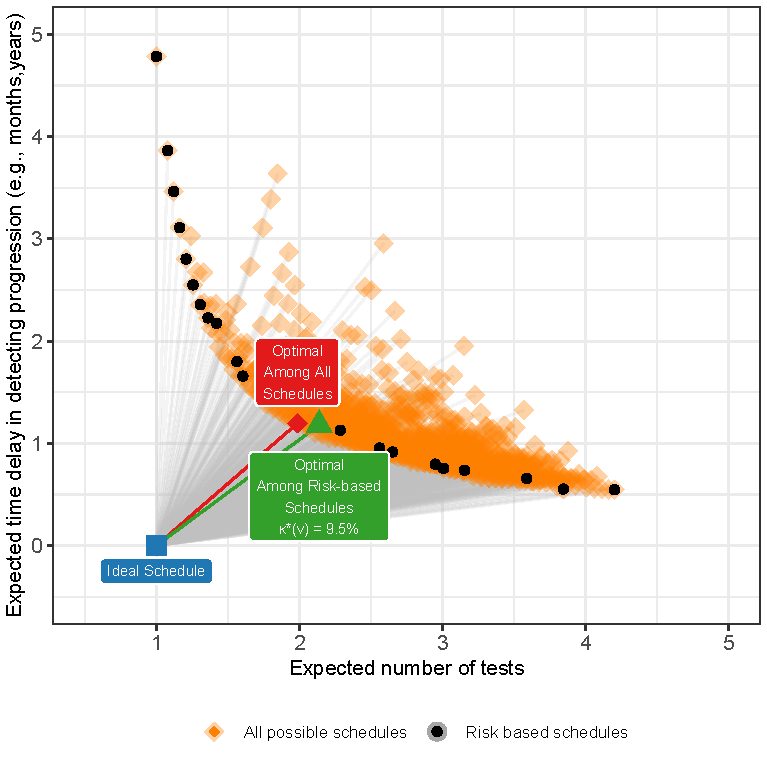
\includegraphics{contents/c4/images/c4_fig_app2.pdf}}
\caption{\textbf{Extension of Figure~\ref{c4:fig:4}, by optimizing the Euclidean distance~(\ref{c4:eq:kappa_choice}) among all possible schedules}. Let~$U = \{u_1, \ldots, u_L\}$ represent a schedule of pre-fixed future visits (e.g., biannual PSA measurement in prostate cancer) on which we wanted to decide for conducting future invasive test. Since each test decision is binary, given~$L$ visits in~$U$, a total of~$2^L$ test schedules can be created (orange Rhombus). Risk-based personalized schedules obtained via~(\ref{c4:eq:personalized_decision_grid}) and shown by black circles, constitute a small subset of these~$2^L$ schedules. Ideal schedule of tests: point (1,0) shown as a blue square. It plans exactly one invasive test at the true time of progression~$T^*_j$ of a patient. That is, zero time delay in detecting progression.}
\label{c4:fig:app2}
\end{figure}

\section{Simulation Study Extended Results}
In the simulation study, we evaluated the following biopsy schedules~\citep{loeb2014heterogeneity, inoue2018comparative}: biopsy every year (annual), biopsy according to the PRIAS schedule (PRIAS), personalized biopsy schedules based on two fixed risk thresholds, namely,~$\kappa=10\%$, and automatically chosen optimal~$\kappa^*(v)$ (Section~\ref{c4:sec:schedule}), and automatically chosen optimal~${\kappa^*\{v \mid E(D)\leq 0.75\}}$ with a constraint of 9 months (0.75 years) on expected delay in detecting progression. Lastly, we added two more optimal schedules to this list. Specifically,~$S^*(v)$ denotes an optimal schedule among all possible schedules (Section~\ref{c4:appendix:all_possible}), and~$S^*\{v \mid E(D)\leq 0.75\}$ is extension of~$S^*(v)$ with a constraint of 9 months (0.75 years) on expected delay in detecting progression.

We compare all the aforementioned schedules on two criteria, namely the number of biopsies they schedule and the corresponding time delay in detection of cancer progression in years (time of positive biopsy - true time of cancer progression). The corresponding results, using~${\mbox{500} \times \mbox{250}}$ test patients are presented in Table~\ref{c4:table:extended_simres}. Since the simulated cohorts are based on PRIAS, roughly only 50\% of the patients progress in the ten year study period. While we are able to calculate the total number of biopsies scheduled in all~$500 \times 250$ test patients, but the time delay in detection of progression is available only for those patients who progress in ten years (\emph{progressing}). Hence, we show the simulation results separately for \emph{progressing} and \emph{non-progressing} patients.

\begin{table}
\small
\centering
\caption{\textbf{Simulation study results for all patients}: Estimated mean ($\mu$), median (Med), first quartile~$\mbox{Q}_1$, and third quartile~$\mbox{Q}_3$ for number of biopsies (nb) and for the time delay (d) in detection of cancer progression in years, for various biopsy schedules. The delay is equal to the difference between the time of the positive biopsy and the simulated true time of progression. Types of schedules:~${\kappa=10\%}$ and~$\kappa^*(v)$ schedule a biopsy if the cumulative-risk of cancer progression at a visit is more than 10\%, and an automatically chosen threshold, respectively. Schedule~${\kappa^*\{v \mid E(D)\leq 0.75\}}$ is an extension of~$\kappa^*(v)$ with a constraint of 9 months (0.75 years) on expected delay in detecting progression.~$S^*(v)$ denotes an optimal schedule among all possible schedules (Section~\ref{c4:appendix:all_possible}), and~$S^*\{v \mid E(D)\leq 0.75\}$ is an extension of~$S^*(v)$ with a constraint of 9 months (0.75 years) on expected delay in detecting progression. Annual corresponds to a schedule of yearly biopsies, and PRIAS corresponds to biopsies as per PRIAS protocol.}
\label{c4:table:extended_simres}
\begin{tabular}{l|rrrr|rrrr}
\toprule
\multicolumn{9}{l}{\textbf{Progressing patients (50\%)}}\\
\midrule
Schedule & $\mbox{Q}_1^{\mbox{nb}}$ & $\mu^{\mbox{nb}}$ & $\mbox{Med}^{\mbox{nb}}$ & $\mbox{Q}_3^{\mbox{nb}}$ & $\mbox{Q}_1^{\mbox{d}}$ & $\mu^{\mbox{d}}$ & $\mbox{Med}^{\mbox{d}}$  & $\mbox{Q}_3^{\mbox{d}}$ \\
\midrule
Annual        & 1  & 3.71 & 3  & 6  & 0.29 & 0.55 & 0.57 & 0.82\\
PRIAS         & 1  & 2.88 & 2  & 4  & 0.38 & 0.92 & 0.74 & 1.00\\
$\kappa=10\%$ & 1  & 2.55 & 2  & 4  & 0.45 & 1.00 & 0.85 & 1.33\\
$\kappa^*(v)$ & 1  & 2.46 & 2  & 3  & 0.45 & 0.89 & 0.86 & 1.26\\
$\kappa^*\{v \mid E(D)\leq 0.75\}$ & 1  & 3.39 & 3  & 5  & 0.32 & 0.61 & 0.63 & 0.88\\
$S^*(v)$ & 1  & 2.07 & 2  & 3  & 0.55 & 1.06 & 1.01 & 1.49\\
$S^*\{v \mid E(D)\leq 0.75\}$ & 1  & 2.79 & 2  & 4  & 0.39 & 0.75 & 0.76 & 1.06\\
\midrule
\multicolumn{9}{l}{\textbf{Non-progressing patients (50\%)}}\\
\midrule
Annual         & 10 & 10.00   & 10 & 10 & - & - & - & -\\
PRIAS          & 4  & 6.40 & 6  & 8  & - & - & - & -\\
$\kappa=10\%$  & 4  & 4.91 & 5  & 6  & - & - & - & - \\
$\kappa^*(v)$  & 6  & 6.22 & 6  & 7  & - & - & - & -\\
$\kappa^*\{v \mid E(D)\leq 0.75\}$ & 8 & 8.68 & 9  & 9  & - & - & - & -\\
$S^*(v)$  & 5  & 6.49 & 5  & 6  & - & - & - & -\\
$S^*\{v \mid E(D)\leq 0.75\}$ & 7 & 7.22 & 7  & 7  & - & - & - & -\\
\bottomrule
\end{tabular}
\end{table}

\section{Partially Observable Markov Decision Processes}
\label{c4:appendix:pomdp}
Partially observable Markov decision processes or POMDPs have been utilized in numerous optimal screening and surveillance test schedules for chronic diseases~\citep{steimle2017markov}, and especially for nearly all types of cancers~\citep{alagoz2010operations}. A notable advantage of POMDPs is that they find an optimal schedule from all schedules possible over a set of follow-up visits. In our case, this means all~$2^L$ possible schedules given visit schedule~$U = \{u_1, \ldots, u_L\}$. To our knowledge, POMDPs and joint models have not been integrated yet. Thus, our aim is to integrate them to make the definition of POMDPs personalized, and then evaluate their strengths and limitations. The components of our discrete-time space POMDP are as follows (subscript~$j$ denotes the subject).

\paragraph{\textbf{Decision epochs}:} The decision epoch~$u \in U$ is the time at which we want to take a decision of an invasive test. These are typically pre-fixed future follow-up visits for biomarker measurements (Section~\ref{c4:subsec:pers_schedule}).

\paragraph{\textbf{Actions}:} Two types actions can be taken at each decision epoch~$u$, namely, an invasive test~$IT$ or waiting until the next decision epoch~$W$. The action taken at time~$u$ is denoted by~${q(u) \in \{IT,W\}}$. The history of all actions taken until time~$u$ is~${Q(u)=\{q(0), \ldots q(u)\}}$.

\paragraph{\textbf{(Disease) States}:} At decision epoch~$u$, the disease state of the patient is denoted by~$s_j(u) \in S$. The vector of all states~$S_j = \{P, NP, R\}$, where~$P$ denotes that the patient has obtained disease progression (event of interest), and~$NP$ denotes that patient has not obtained progression. Unlike progression~$P$ and not progression~$NP$, the third state~$R$ called removal from surveillance, is observable. Removal of a patient from surveillance occurs only after progression~$P$ has been observed. The state~$R$ is also an absorbing state, and hence it always transitions to itself, irrespective of the action taken. 

In joint modeling terms, ~$s_j(u)=NP$ is equivalent to~$T^*_j > u$ (right-censored), and~$s_j(u) = P$ means ~$u^- < T^*_j \leq u$ (interval-censored), where ${u^- = \mbox{max}\{v \mid s_j(v) = NP, v < u\}}$ is the time of the last visit on which an invasive test was conducted to confirm that the patient had not progressed.

\paragraph{\textbf{Observations}:} We cannot observe the underlying disease states~$P$ and~$NP$ unless we take the action invasive test~$IT$. However, the disease state is manifested by observable clinical data, e.g., PSA and DRE in prostate cancer. Specifically, we can observe a~$K$-tuple of clinical data~$\boldsymbol{y}_j(u) = \{y_{1j}(u),\ldots y_{Kj}(u)\}$ on each decision epoch~$u$ to guide our actions. When the patient is in state~$R$ (removed from surveillance) a special observation tuple~$\boldsymbol{y}_j(u)=(\phi,\ldots,\phi)$, denoting empty data, is observed. The observation history at time~$u$ is given by~${\mathcal{Y}_j(u) = \{\boldsymbol{y}_j(0) \ldots \boldsymbol{y}_j(u)\}}$. 

Typically POMDPs make two assumptions about clinical observations. First, that observations are categorical in nature. This is done to avoid the curse of dimensionality. Second, at any time $u-1$ the probability distribution of future observations $p\{\boldsymbol{y}_j(u) \mid s_j(u)\}$ is assumed independent of the observation history. This means that probability distribution of future observations adds unique information over observed data. Conversely, in the joint modeling framework continuous observations are allowed, and probability distribution of future observation $p\{\boldsymbol{y}_j(u) \mid \boldsymbol{b}_j\}$ depends entirely on the patient-specific random effects $\boldsymbol{b}_j$ that are estimated from the observed data $p\{\boldsymbol{b}_j \mid s_j(u), \mathcal{Y}_j(u-1)\}$. That is, the probability distribution of future observations adds no extra value over observed data and current disease state. Hence, hereafter we denote longitudinal data history as $\mathcal{Y}_j$ and do not specify the time up to which it is observed.

\paragraph{\textbf{Belief}:} The states~$P, NP$ cannot be observed directly. In this regard, our belief regarding what state the patient is in, is given by the corresponding probability of being in a certain state. The vector of these probabilities is called the belief vector. It is given by,
\begin{equation*}
\begin{split}
\pi_j(u) = \Big[& \mbox{Pr}\big\{s_j(u)=P \mid \mathcal{Y}_j, Q(u-1)\big\}, \\
& \mbox{Pr}\big\{s_j(u)=NP \mid \mathcal{Y}_j, Q(u-1)\big\},\\
&\mbox{Pr}\big\{s_j(u)=R \mid \mathcal{Y}_j, Q(u-1)\big\}\Big].
\end{split}
\end{equation*} 
The sum ~$\sum_{s_j(u) \in S} \mbox{Pr}\{s_j(u) \mid \mathcal{Y}_j, Q(u-1)\} = 1$ of these probabilities is always equal to one. Since the state~$R$ removed from surveillance can be observed directly, $\mbox{Pr}\{s_j(u)=R \mid \mathcal{Y}_j, Q_j(u-1)\} \in \{0,1\}$.

The belief vector is calculated on the basis of both the current observation, previous belief, latest action, and transition probabilities from previous state to current state. To this end, POMDPs utilize the Bayes rule~\citep{steimle2017markov}. In contrast, in joint modeling framework the disease state distribution is estimated as random-effects, and subsequently the belief is expressed as the probability distribution of the time to event outcome. Specifically, 

\begin{equation}
\label{c4:eq:belief_jm}
\begin{split}
\mbox{Pr}\big\{s_j(u)=NP \mid \mathcal{Y}_j, Q(u-1)\big\} &= \mbox{Pr}(T^*_j > u \mid T^*_j>u^-, \mathcal{Y}_j),\\
\mbox{Pr}\big\{s_j(u)=P \mid \mathcal{Y}_j, Q(u-1)\big\} &= \mbox{Pr}(T^*_j \leq u \mid T^*_j>u^-, \mathcal{Y}_j).
\end{split}
\end{equation} 

\paragraph{\textbf{Transition Probabilities}:} Patient's disease state changes over follow-up, and also with actions. For example, if an action~$q(u)=IT$ is taken when the patient is in state~$s_j(u)=P$, then the state at next decision time $u+1$ is removal from surveillance, i.e,~${s_j(u+1)=R}$. However, if~$s_j(u)=NP$, then invasive test action $IT$ or waiting $W$ do not change state. This is because, disease transition from not progressed to progressed is a natural process, and not altered by invasive tests. Transition from one state to another happens with a certain probability. This probability can be obtained from the joint model, as shown in Table~\ref{c4:table:state_transition}.
\begin{table}[htb]
\small
\centering
\caption{State transition matrix for a POMDP}
\label{c4:table:state_transition}
\begin{tabular}{l|ccc} 
\toprule
\multicolumn{4}{l}{\textbf{Action: Invasive Test $q(u)=IT$}}\\
 \midrule
$\pi_j(u+1)$ & $s_j(u)=NP$ & $s_j(u)=P$ & $s_j(u)=R$\\
 \midrule
 ~$s_j(u+1)=P$ &$1 - \mbox{Pr}(T^*_j > u+1 \mid T^*_j >u, \mathcal{Y}_j)$ & 0  & 0 \\
~$s_j(u+1)=NP$ & $\mbox{Pr}(T^*_j > u+1 \mid T^*_j >u, \mathcal{Y}_j)$ & 0 & 0 \\
 ~$s_j(u+1)=R$ & 0 & 1 & 1 \\
  \midrule
 \multicolumn{4}{l}{\textbf{Action: Waiting $q(u)=W$}}\\
 \midrule
 $\pi_j(u+1)$ & $s_j(u)=NP$ & $s_j(u)=P$ & $s_j(u)=R$\\ 
 \midrule
 ~$s_j(u+1)=P$ & $1 - \mbox{Pr}(T^*_j > u+1 \mid T^*_j >u, \mathcal{Y}_j)$ & 1 & 0 \\
~$s_j(u+1)=NP$ & $\mbox{Pr}(T^*_j > u+1 \mid T^*_j >u, \mathcal{Y}_j)$ & 0 & 0 \\
  ~$s_j(u+1)=R$ & 0 & 0 & 1 \\
\bottomrule
\end{tabular}
\end{table}

The state transition matrix in Table~\ref{c4:table:state_transition} can also be seen as a belief transition matrix. Specifically, given the current state $s_j(u)$ and history of actions $q(u)$ we can obtain a new belief. For example, if $s_j(u)=NP$, and $q(u)=IT$ then belief vector at next epoch $u+1$ is given by:
\begin{equation}
\label{c4:eq:belief_transition}
\begin{split}
\pi_j\big\{u+1 \mid s_j(u)=NP, q(u)=IT\big\} = \Big[ & 1 - \mbox{Pr}(T^*_j > u+1 \mid T^*_j >u, \mathcal{Y}_j),\\
& \mbox{Pr}(T^*_j > u+1 \mid T^*_j >u, \mathcal{Y}_j), 0\Big].
\end{split}
\end{equation}

\paragraph{\textbf{Reward}:} The criterion of optimality in POMDPs is the weighted cumulative reward. A reward is a number that is chosen manually for four possible outcomes (true-positive, false-positive, true-negative, and false-negative) of a binary test/no test decision in a schedule. The weighted cumulative reward of a schedule is the weighted sum of all rewards possible with all sequential test decisions in a schedule. Let us assume the following immediate rewards for action $q(u)$, conditional on knowing the state of the patient and the data. These are denoted by $B\{q(u) \mid s_j(u)\}$ and exemplified in Table~\ref{c4:table:rewards}.
\begin{table}[htb]
\small
\centering
\caption{Reward matrix for a POMDP}
\label{c4:table:rewards}
\begin{tabular}{l|cc} 
 \toprule
  & $q(u)=IT$ & $q(u)=W$ \\
  \midrule
 $s_j(u)=NP$ & a (unnecessary test) & b (saved unnecessary test) \\
  $s_j(u)=P$ & c (correct test) & d (skipped necessary test) \\
  $s_j(u)=R$ & 0 & 0 \\
\bottomrule
\end{tabular}
\end{table}
Since the state of the patient is unobservable, the weighted reward of an action at time $u$ is:

\begin{equation*}
B\big\{q(u) \mid \pi_j(u)\big\} = \sum_{s \in S} B\big\{q(u) \mid s_j(u) = s\big\} \mbox{Pr}\big\{s_j(u) = s \mid \mathcal{Y}_j, Q(u-1)\big\}.
\end{equation*}
The weights $\mbox{Pr}\big\{s_j(u) = s \mid \mathcal{Y}_j, Q(u-1)\big\}$ are defined in~(\ref{c4:eq:belief_jm}). 

\paragraph{\textbf{Dynamic Programming Equations}:}
The dynamic programming equations for our POMDP, starting from a belief $\pi_j (u)$ at time $u$ is given by (condition on observed data $\mathcal{Y}_j(u)$ and action history $Q(u-1)$ is dropped for brevity, but assumed):
\begin{equation*}
\begin{split}
    V\big\{\pi_j(u)\big\} &= B\big\{q^*(u) \mid \pi_j(u) \big\} + \rho \sum_{s \in S} \mbox{Pr}\big\{s_j(u) = s \mid \mathcal{Y}_j(u), Q(u-1)\big\}\\
    & \quad \quad\quad\quad\quad\quad \quad \quad \times V\big[\pi_j\{u+1 \mid s_j(u)=s, q^*(u)\}\big],\\
     q^*(u) &= \underset{q(u) \in \{IT,W\}}{\mbox{arg max}} \Big\{B\big\{q(u) \mid \pi_j(u) \big\} + \rho \sum_{s \in S} \mbox{Pr}\big\{s_j(u) = s \mid \mathcal{Y}_j(u), Q(u-1)\big\}\\
    & \quad \quad\quad\quad\quad\quad \quad \quad \times V\big[\pi_j\{u+1 \mid s_j(u)=s, q(u)\}\big]\Big\}
\end{split}
\end{equation*}
where $0 \leq \rho \leq 1$ is the discount factor with the interpretation that it is the probability of rewards at and after time $u$ being useful, and future belief $\pi_j\{u+1 \mid s_j(u)=s, q(u)\}$ is defined in~(\ref{c4:eq:belief_transition}).

\subsection{Choice of Reward Function for POMDPs}
Consider the scenario that patient has not been detected in progressed $P$ state yet. That is, there is zero probability of being the third state $R$ called removed from surveillance. In this scenario, the belief vector at any time $u$ is given by $\pi_j(u) = (p, 1-p, 0)$, where $p=\mbox{Pr}\big\{s_j(u)=P \mid \mathcal{Y}_j(u), Q(u-1)\big\}$ is the probability that the patient is currently in state $P$. If we calculate the weighted reward of a single action (that is not looking ahead in time), it is given by,
\begin{equation}
\label{c4:eq:reward_IT_W}
\begin{split}
B\big\{q(u)=IT\big\} &= c\times p + a \times (1-p),\\
B\big\{q(u)=W\big\} &= d\times p + b \times (1-p).
\end{split}
\end{equation}
The action invasive test $IT$ will be taken if reward of test is more than reward of waiting, i.e., $B\big\{q(u)=IT\big\} > B\big\{q(u)=W\big\}$. Thus using~(\ref{c4:eq:reward_IT_W}), we can say that if $p > (b-a)/(c-d + b-a)$, then action $IT$ will be taken. The right hand side $(b-a)/(c-d + b-a)$ is a constant. Infinite combinations of rewards $a,b,c,d$ can satisfy the condition $p > (b-a)/(c-d + b-a)$. Typically POMDP rewards are chosen based on survey results~\citep{steimle2017markov} and translated as quality-adjusted life-years (QALY) saved. However, the main concern is that with infinite optimal reward sets, any reward set can be cherry-picked, including those that correspond to (improbable) thousands of quality-adjusted life-years saved. Besides the estimates for QALYs are usually not personalized before use in the model.

\section{Source Code}
\label{c4:appendix:source_code}
The source code for reproducing results of this chapter is available at \url{https://github.com/anirudhtomer/PersonalizedSchedules}.
\end{subappendices}